%------------------------------------------------------------------------
% Chapter:  PDF calculation
%------------------------------------------------------------------------

\chapter{Atomic pair distribution function \label{pdf}}

The atomic pair distribution function (PDF) can be obtained from
powder diffraction data and is a valuable tools for the study of the
{\it local} atomic arrangements in a material. This chapter
describes how \Discus can be used to calculate and refine a
PDF. 
In real space the PDF of a given
structure can be calculated using the relation:
%
\begin{equation}
  G_{c}(r) = \frac{1}{r} \sum_{i}\sum_{j} \left [
             \frac{b_{i}b_{j}}{\langle b \rangle ^{2}}
             \delta (r - r_{ij}) \right ]   - 4 \pi r \rho_{0},
  \label{eq_igr}
\end{equation}
%
where the sum runs over all pairs of atoms $i$ and $j$ within the
model crystal separated by $r_{ij}$. The scattering power of atom
$i$ is $b_{i}$ and $\langle b \rangle$ is the average scattering
power of the sample. In case of neutron scattering $b_{i}$ is simply
the scattering length, in case of X-rays it is the atomic form
factor evaluated at a user define value of $Q$. The default value is
$Q=0$ in which case $b_{i}$ is simply the number of electrons of
atom $i$. 

As this calulation in direct space is an approximation that can be rather crude 
for X-rays and electrons,
see \cite{nepr2021}, \Discus uses a different algorithm to calculate the 
PDF. 

Once you have build a model structure, use the powder menu to calculate
a powder diffraction pattern. Within the output menu \Discus offers the 
possibility to write the powder diffraction pattern in may different
formats, as well as an option to write the PDF. Essentially \Discus
does the same as you will have done in an experiment. First the sample
is  subject to the Fourier transform to calculate the powder diffraction 
pattern and then this pattern is transformed back into direct space 
via a fast sine-Fourier transform.





%------------------------------------------------------------------------

\section{Calculating the PDF \label{pdf-calc}}

The PDF can be calculated for extended crystals as well as nanoparticles.
For extended crystals it is usually faster to use the complete integration
mode as described in section \ref{four-powder} and in the on-line help.
For nanoparticles, the Debye-Scattering-Equation is well adapted.

The first example illustrates the effect of instrumental resolution on the 
PDF. The powder pattern of Nickel was calculated using the complete integration
technique in both cases. Figure \ref{pdf-fig1} shows the Nickel PDF and 
the diffraction pattern calculated with high angular resolution. As
is expected, the peaks in the PDF extend with significant height over
a large distance range, way beyond the 100\AA{} shown in the Figure.
%
\begin{figure}[!b]
   \centering
   \includegraphics[scale=0.5, angle=270]{pdf1.eps}
   \vspace*{+20mm}
   \caption{Calculated PDFs of $Ni$. High angular resolution was 
             assumed for the powder pattern.}
   \label{pdf-fig1}
\end{figure}
%
Figure 2 \ref{pdf-fig2} shows the corresponding pattern for an instrument with much 
broader instrumental resolution, compareable to many PDF beam lines
at synchrotron sources. The observed Bragg reflections are much wider 
and the peaks in the PDF decrease rapidly with increasing distance r.
%
\begin{figure}[!b]
   \centering
   \includegraphics[scale=0.5, angle=270]{pdf2.eps}
   \vspace*{+20mm}
   \caption{Calculated PDFs of $Ni$. Broad angular resolution was 
             assumed for the powder pattern, as commonly used at PDF beam lines.}
   \label{pdf-fig2}
\end{figure}
%
\par
The effect of a finite Q-range is illustrated in Figure \ref{pdf-fig3}. Here 
the powder pattern were calculated to Q$_{max}$ = 50, 20 and 15\AA$^{-1}$, 
respectively. For the smaller Q$_{max}$ values the width of the PDF peak
increases and the finite Fourier ripples become more pronounced.
%
\begin{figure}[!b]
   \centering
   \includegraphics[scale=0.5, angle=270]{pdf3.eps}
   \vspace*{+20mm}
   \caption{Calculated PDFs of $Ni$. Effect of different Q$_{max}$ values.
             Blue: 50\AA$^{-1}$; red: 20\AA$^{-1}$; black: 15\AA$^{-1}$.}
   \label{pdf-fig3}
\end{figure}
%

\begin{MacVerbatim}
  1 variable real, P_u
  2 variable real, P_v
  3 variable real, P_w
  4 variable real, P_eta
  5 variable real, P_qmax
  6 P_u = 0.0000
  7 P_v = 0.0000
  8 P_w = 0.0050
  9 P_eta = 0.5000
 10 P_qmax = 20.000
 11 #
 12 read
 13 cell CELL/nickel.cell
 14 #
 15 powder                          # Switch to powder menu
 16   reset
 17   xray                          # Select X-rays
 18   set axis,q                    # Perform calculation on equaly spaced Q grid
 19   set calc,complete             # Use complete integration algorithm-algorithm
 20   set disp,off                  # Switch anomalous dispersion off
 21   set delta,0.0                 # Set simple convolution by Gaussian off
 22   set qmin,0.5500               # Starting value for Q
 23   set qmax,P_qmax               # Final value for Q
 24   set dq,  0.0010               # Step size for Q
 25   set dh, 1.0                   # Step sizes HKL
 26   set dk, 1.0
 27   set dl, 1.0
 28   set profile, off              # Switch convolution by Pseudovoigt function off
 29   set profile, pseudo           # Use Pseudovoigt (instead of Gaussian)
 30   set profile, uvw, P_u, P_v, P_w # Cagliotti u,v,w values 
 31   set profile, eta, P_eta       # Mixing parameter 1=Lorenzian 0=Gaussian
 32   set profile, asym, 0.00, 0.00, 0.00, 0.00 # Asymmetry parameters
 33   set temp,use                  # Use the Atomic displacement parameters
 34   set wvle,0.20000              # Set the wavelength
 35   set four,four                 # Just for stacking fault mode, set to normal
 36   set lpcor,bragg, 2.00         # Define Lorentz-Pol to BraggBrentano Diffractometer
 37   run                           # Do the actual calculation
 38 exit                            # Go back to main DISCUS menu
 39 #
 40 output                          # Switch to output menu
 41   value inte                    # Select intensity as output value
 42   outf  "POWDER/complete_%52F.inte", P_qmax   # Define output file name
 43   form  powder,q                # Write output as powder data
 44   run                           # Perform the actual output
 45
 46   value PDF                     # Select intensity as output value
 47   outf  "PDF/complete_%5.2F.grcalc", P_qmax   # Define output file name
 48   form  pdf, r,0.01, 100.0, 0.01  # Write output as powder data
 49   run                           # Perform the actual output
 50 exit                            # Go back to main DISCUS menu
\end{MacVerbatim}
%
The macro file used to calculate the Nickel PDFs is listed above.
In the first 10 lines, the variables for the profile function are defined
and given appropriate values. As the calculation used the complete
integration, a single unit cell is sufficient (lines 12/13). 
Lines 15 to 38 define the powder diffraction pattern. The pattern is
calculated for xrays (line 17), using the complete integration mode, line(19)
Since we have a single unit cell steps in reciprocal space are limited to intger 
HKL, lines 25-27. The variable {\tt P\_qmax} is used in line 23 to set the 
upper Q limit. The powder pattern is convoluted with a Pseudo-Voigt function,
lines 28 to 32. In this example a constant eta value is use, but note that \Discus
allows a linear and squre Q dependence of eta as well. Noasymmetry is used in 
this simple example.

Lines 40 to 50 write the output. Lines 41 to 44 write the intensity on a Q-scale.
Here the Q-max parameter is used to create a flexible file name.

To write the PDF, \Discus uses the output menu as well. In line 46 the output
is defined to be a powder PDF {\tt value PDF}. Capitalization of {\tt PDF} is
mandatory. Line 48 defines the output format to be a PDF on a distance scale
in (optional) limits from 0.01\AA{} to 100.0\AA{} in steps of 0.01\AA.
At the run command in line 49, \Discus will internally perform the transformation
of the powder pattern into a powder PDF.


%------------------------------------------------------------------------

\section{Refining a PDF \label{pdf-rmc}}

To refine an experimental model against a PDF, you can use the two 
refinement algorithms build into the \Suite. Alternatively the 
Reverse Monte Carlo (RMC) algorithm can be used as well.

Essentially you would create the model structure based on a parameter set, 
calculate the powder diffraction pattern and write the PDF using the 
output menu as decribed in the previous section. 
\par
! to be revised !, example to come
\par
%In principle an experimental PDF can be refined based on a
%structural model in two different ways. A relatively small model can
%be refined using {\it PDFFIT}. On the other hand a larger model can
%be refined using the Reverse Monte Carlo (RMC) algorithm in 
%\discus. Details about the principle of RMC are discussed in chapter
%\ref{rmc} of this manual. The only difference is that rather than
%refining the scattering intensity directly, the PDF is refined. An
%example refinement of a Nickel PDF is listed below and is also part
%of the online tutorial of \discus.
%%
%
%\begin{MacVerbatim}
%      1 read
%      2 cell ni.stru
%      3 #
%      4 pdf
%      5   data ni.data
%      6 #
%      7   set frange,1.5,10.0
%      8   set qmax,22.0
%      9   set rad,xray
%     10   sel ni
%     11   set mode,shift
%     12   set move,ni,0.01,0.01,0.01
%     13   set disp,1
%     14   set cyc,25
%     15   show all
%     16   run
%     17   save pdf,rmc.pdf
%     18   save stru,rmc.stru
%     19 exit
%\end{MacVerbatim}
%%
%In lines 1--2 the starting structure is read. Next the {\tt pdf}
%sub level is entered (line 4). First we read the observed PDF from
%the file {\it ni.data}. The maximum $r$ and $\Delta r$ which defines
%the range of the calculated PDF are taken from the data file just
%read. Then the range in $r$ that actually should be used for the
%refinement is set (line 7), here from 1.5 to 10.0\AA. In lines 8--9
%the value of $Q_{max}$ and the radiation used in the experiment is
%set. Now we enter the RMC related settings (see also \ref{rmc}). We
%select atoms to be moved (line 10), here Ni. This command should not
%be confused with {\tt isel} or {\tt jsel} which actually selects the
%atoms that are included in the calculation of the PDF. The RMC mode
%is set to shift atoms using a Gaussian distribution with a sigma of
%0.01 lattice units ($\approx 0.035$\AA) in lines 11--12. Finally we
%set the screen update interval to 1 (line 13) and specify that 25
%cycles will be carried out (line 14). Before the refinement is
%started in line 16, the current settings are displayed using the
%command {\tt show} (line 15). After the refinement is finished, the
%resulting PDF (line 17) and structure (line 18) is saved to a file.
%\par

%------------------------------------------------------------------------
